\cotefile{148}
\scanpage{8}

\begin{minipage}[c]{.43\linewidth}\centering
U N I V E R S I T E\\
DES SCIENCES ET TECHNIQUES\\
\begin{tabular}{@{}l@{}}
\texttt{DU LANGUEDOC}\\[-.6ex]
\texttt{-{}-{}-{}-{}-{}-{}-{}-{}-{}-{}-{}-}
\end{tabular}

Service de la Scolarité\\
MA/GJ\\
Diffusion : Liste A\\
N° : 4679
\end{minipage}\hfill
\begin{minipage}[c]{.54\linewidth}\raggedleft
Montpellier, le 20 octobre 1983
\end{minipage}


\begin{center}
\begin{tabular}{@{}l@{}}
\texttt{AVIS DE SOUTENANCE D'UNE THESE DE DOCTEUR INGENIEUR}\\[-.6ex]
\texttt{-{}-{}-{}-{}-{}-{}-{}-{}-{}-{}-{}-{}-{}-{}-{}-{}-{}-{}-{}-{}-{}-{}-{}-{}-{}-{}-{}-{}-{}-{}-{}-{}-{}-{}-{}-{}-{}-{}-{}-{}-{}-{}-{}-{}-{}-{}-{}-{}-{}-{}-{}-}
\end{tabular}

\begin{tabular}{@{}l@{}}
\texttt{AUTOMATIQUE}\\[-.6ex]
\texttt{-{}-{}-{}-{}-{}-{}-{}-{}-{}-{}-}
\end{tabular}
\end{center}

\uline{Nom et prénom du candidat} : SITOHANG Benhard

\uline{Titre de la thèse} : LINAIRE : SYSTEME DE GESTION DE BASES DE DONNEES RELATIONNELLES SUR MICRO-ORDINATEUR.

\uline{Date, heure et lieu de soutenance prévus:} 28 OCTOBRE 1983 à 14h30 - CRIG USTL

\uline{Nom du Directeur de thèse} : Monsieur le Professeur B. FILLIATRE

\uline{Désignation du laboratoire où la thèse est préparée} : CRIG USTL

\uline{Résumé de la thèse} :

La conception et la réalisation d'un Système de Gestion de Bases de Données Relationnelles sur micro-ordinateur, que nous avons baptisé ``LINAIRE'', est le sujet de cette thèse.

Nous mettons l'accent sur trois points principaux :

1. BOUCLE MULTI-NIVEAUX ; c'est une technique du traitement de données, permettant d'éviter l'utilisation des relations intermédiaires comme résultats des opérateurs relationnels, ce qui serait particulièrement pénalisant pour un micro-ordinateur possédant une mémoire centrale limitée.

2. STRUCTURE INTERNE DE LA BASE ; elle est multiple, afin de préserver au mieux les performances tout en offrant en particulier la possibilité d'accélérer le traitement de l'opérateur relationnel ``équi-joint''.

3. L'adaptation sur un micro-ordinateur du langage de manipulation de QUERY-BY-EXAMPLE (langage de haut niveau, interactif, et tabulaire).

\uline{Durée approximative des recherches ayant abouti à la thèse} : 2 ans

\uline{Composition du jury proposé} :

\begin{tabular}{ll}
MM. & FILLIATRE B.\\
& CHEIN M.\\
& PICHAT E.\\
& PIROTTE A.\\
& PRUNET F.
\end{tabular}

\begin{center}
P. le Secrétaire Général,\\
l'Attachée Principale d'Administration Scolaire\\
et Universitaire,

\figure{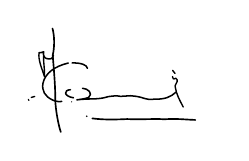
\begin{tikzpicture}[x=.014cm,y=-.014cm,line cap=round,line join=round]
\draw[line width=.6pt] (48.6,8.7) .. controls (50.7,16.1) and (50.4,26.6) .. (48.8,32.9)
  .. controls (49.7,44.2) and (51.3,61.7) .. (51.1,73.8)
  .. controls (51.5,83.0) and (53.9,96.0) .. (56.1,102.5);
\draw[line width=.55pt] (36.5,30.7) .. controls (38.0,31.7) and (40.3,29.2) .. (40.6,29.8)
  .. controls (39.7,32.8) and (41.4,35.7) .. (43.4,36.0)
  .. controls (46.8,36.8) and (48.8,36.2) .. (49.4,33.0);
\draw[line width=.5pt] (36.5,30.7) .. controls (35.3,36.5) and (38.9,44.8) .. (41.4,52.5)
  .. controls (41.8,46.6) and (40.2,39.8) .. (40.6,33.7);
\draw[line width=.55pt] (62.9,40.0) .. controls (50.2,43.1) and (42.0,49.3) .. (40.0,58.2)
  .. controls (38.7,65.0) and (41.6,70.3) .. (48.7,73.5)
  .. controls (51.6,75.0) and (55.0,75.2) .. (57.0,74.8);
\draw[line width=.55pt] (66.4,39.9) .. controls (74.5,39.8) and (79.8,41.6) .. (80.3,44.8);
\draw[line width=.55pt] (64.9,64.2) .. controls (58.8,64.4) and (58.3,70.0) .. (67.6,71.5);
\draw[line width=.55pt] (75.8,62.9) .. controls (80.7,63.0) and (85.7,67.6) .. (81.4,71.2)
  .. controls (78.2,72.5) and (73.4,72.9) .. (70.7,73.4)
  .. controls (82.8,71.8) and (89.5,73.6) .. (99.0,70.5)
  .. controls (102.3,70.9) and (103.5,69.0) .. (106.7,69.7)
  .. controls (110.7,71.3) and (117.8,68.6) .. (124.5,70.2)
  .. controls (131.0,71.0) and (133.3,73.8) .. (140.4,72.8)
  .. controls (150.8,73.0) and (155.6,70.9) .. (160.7,66.3);
\draw[line width=.5pt] (157.5,46.7) -- (159.7,49.4);
\draw[line width=.5pt] (157.4,52.3) .. controls (158.1,56.2) and (159.6,53.5) .. (160.4,53.8)
  .. controls (163.0,55.1) and (161.1,58.4) .. (160.2,59.7)
  .. controls (159.1,60.3) and (160.5,63.9) .. (161.0,66.5)
  .. controls (162.8,72.3) and (166.0,77.4) .. (167.1,79.9);
\draw[line width=.5pt] (29.4,71.2) -- (32.4,70.3);
\draw[line width=.4pt] (26.6,72.9) -- (27.3,74.0);
\fill (66.0,75.2) circle[radius=.55];
\fill (79.6,88.3) circle[radius=.8];
\draw[line width=.6pt] (84.7,90.2) .. controls (96.1,91.7) and (107.2,91.2) .. (116.4,90.8)
  .. controls (128.7,91.5) and (139.7,90.3) .. (150.2,91.0)
  .. controls (160.7,90.2) and (169.1,91.3) .. (178.1,91.6);
\node[anchor=west] at (184,78) {\unsure{}};
\end{tikzpicture}}

A. GENTIL
\end{center}

\margin{7}
